\section{The Standard Model of Particle Physics}

%%%%%%%%%%%%%%%%%%%%%%%%%%%%%%%%%%
\subsection{Particle Interactions}
%%%%%%%%%%%%%%%%%%%%%%%%%%%%%%%%%%

Interactions between quarks and leptons are described by the \emph{Standard Model of particle physics} (SM). The Standard Model unifies
the electromagnetic and weak forces in a theory of \emph{electroweak interactions} \cite{Glashow:1961tr,*Weinberg:1967tq,*Salam:1968rm},
while strong interactions are described separately by \emph{Quantum Chromodynamics} (QCD) \cite{Fritzsch:1973pi}. Both theories are
based on quantum field theory, in which quarks and leptons are described as fields that interact via bosonic fields.

In the electroweak model there are four vector bosons that mediate interactions, three of which acquire a mass through the
\emph{Brout-Englert-Higgs} (BEH) \emph{mechanism} \cite{Englert:1964et,*Higgs:1964ia,*Higgs:1964pj,*Guralnik:1964eu}. Generating particle
masses this way implies the existence of the scalar \emph{Higgs boson}, which was recently discovered
\cite{Aad:2012tfa,*Chatrchyan:2012ufa}. The BEH mechanism is believed to be also responsible for generating the masses of quarks and
leptons.

The three massive vector bosons are the W$^+$, the W$^-$ and the Z$^0$. These particles are the carriers of the weak interaction. The
remaining massless vector boson is the photon, which mediates the electromagnetic interaction.

Contrary to leptons, quarks carry the ``charge'' of the strong force, or \emph{colour}. This makes them subject to strong interactions,
described by QCD. The mediators of the strong interaction are gluons, which come in eight different types and are coloured particles
themselves.

One of the features of the strong force is that it becomes weaker with increasing interaction energy. This phenomenon is called
\emph{asymptotic freedom} \cite{Gross:1973id,*Politzer:1973fx}. The increasing interaction strength with decreasing energy (or,
equivalently, larger interaction distance) makes it impossible to completely separate coloured particles. As a result, quarks and gluons
are \emph{confined} within colour-neutral objects, such as hadrons.

Whenever possible, \emph{perturbation theory} is used to do calculations of particle interactions. Amplitudes for interaction processes are
expanded as a series in powers of the coupling strength of the interaction. If the coupling strength is small, the exact solution of the
calculation can be approximated by the leading terms in the series. In QCD this only works for high-energy processes, where the strong
force is weak. For low-energy QCD processes, like interactions between quarks inside hadrons, the series diverges and non-perturbative
methods have to be applied.


%%%%%%%%%%%%%%%%%%%%%%%%%%%%%%%%%%
\subsection{Quark-Flavour Physics}
%%%%%%%%%%%%%%%%%%%%%%%%%%%%%%%%%%

Both quarks and leptons come in different \emph{flavours}, which are ordered in three generations (Table~\ref{tab:quarksLeptons}). Unlike
the other interactions, the weak interaction that is mediated by the charged W bosons changes the flavour of a quark or a lepton
\cite{Cabibbo:1963yz,Glashow:1970gm,Kobayashi:1973fv}. This is shown in Figure~\ref{fig:WCouplings} for quarks.
\begin{table}[hbt]
  \begin{tabular}{rccc}
    \hline
                      &  1st generation         &  2nd generation    &  3rd generation    \\
    \hline
    down-type quarks  &  down (d)               &  strange (s)       &  beauty (b)        \\
    up-type quarks    &  up (u)                 &  charm (c)         &  top (t)           \\
    charged leptons   &  electron ($\lepe[-]$)  &  muon ($\lmu[-]$)  &  tau ($\ltau[-]$)  \\
    neutrinos         &  $\nue$                 &  $\numu$           &  $\nutau$          \\
    \hline
  \end{tabular}
  \caption{Quarks and leptons.}
  \label{tab:quarksLeptons}
\end{table}
\begin{figure}[hbt]
  %%BoundingBox: -1 -1 61 36 
%%HiResBoundingBox: -1 -1 60.7757 35.86916 

\hspace*{0.03\textwidth}
\begin{fmffile}{graphics/feynman/WCouplings/up}
  \fmfframe(8,16)(8,16){
    \begin{fmfgraph*}(60,35)
      \fmfstraight
      \fmftop{id,ou}
      \fmfbottom{iW}
      \fmf{fermion}{id,v,ou}
      \fmf{boson}{iW,v}
      \fmflabel{d$_\text{L}^\prime$}{id}
      \fmflabel{u$_\text{L}$}{ou}
      \fmflabel{W}{iW}
    \end{fmfgraph*}
  }
\end{fmffile}
\hfill
\begin{fmffile}{graphics/feynman/WCouplings/charm}
  \fmfframe(8,16)(8,16){
    \begin{fmfgraph*}(60,35)
      \fmfstraight
      \fmftop{id,ou}
      \fmfbottom{iW}
      \fmf{fermion}{id,v,ou}
      \fmf{boson}{iW,v}
      \fmflabel{s$_\text{L}^\prime$}{id}
      \fmflabel{c$_\text{L}$}{ou}
      \fmflabel{W}{iW}
    \end{fmfgraph*}
  }
\end{fmffile}
\hfill
\begin{fmffile}{graphics/feynman/WCouplings/top}
  \fmfframe(8,16)(8,16){
    \begin{fmfgraph*}(60,35)
      \fmfstraight
      \fmftop{id,ou}
      \fmfbottom{iW}
      \fmf{fermion}{id,v,ou}
      \fmf{boson}{iW,v}
      \fmflabel{b$_\text{L}^\prime$}{id}
      \fmflabel{t$_\text{L}$}{ou}
      \fmflabel{W}{iW}
    \end{fmfgraph*}
  }
\end{fmffile}
\hspace*{0.03\textwidth}

  \caption{Charged-current weak interactions of quarks.}
  \label{fig:WCouplings}
\end{figure}

Down-type quarks couple to up-type quarks in the interaction with a W boson. Only quarks with a left-handed chirality participate in this
interaction, which is why the quarks in Figure~\ref{fig:WCouplings} carry a subscript ``L''.

The primes on the d$_\text{L}^\prime$, s$_\text{L}^\prime$ and b$_\text{L}^\prime$ quarks in the figure indicate that the states that
couple to the W boson are not the quark mass eigenstates. The down-type states in the interaction are given by a rotation of the mass
eigenstates, which is parameterized by the Cabibbo-Kobayashi-Maskawa (CKM) quark-mixing matrix \cite{Kobayashi:1973fv}:
\begin{equation}
  \begin{pmatrix} \text{d}_\text{L}^\prime \\ \text{s}_\text{L}^\prime \\ \text{b}_\text{L}^\prime \end{pmatrix}
    \equiv \VCKM\, \begin{pmatrix} \text{d}_\text{L} \\ \text{s}_\text{L} \\ \text{b}_\text{L} \end{pmatrix}
    \equiv \begin{pmatrix} \Vud & \Vus & \Vub \\ \Vcd & \Vcs & \Vcb \\ \Vtd & \Vts & \Vtb \end{pmatrix}
           \begin{pmatrix} \text{d}_\text{L} \\ \text{s}_\text{L} \\ \text{b}_\text{L} \end{pmatrix}
    \ .
\end{equation}
Mixing of lepton states is described by a similar mechanism \cite{Pontecorvo:1957cp,*Pontecorvo:1957qd,*Maki:1962mu,*Pontecorvo:1967fh}.

The CKM matrix is a unitary complex matrix. The number of independent parameters in the matrix is limited by the constraint of unitarity
and by the fact that part of the complex phases of the matrix elements can be absorbed in the arbitrary phases of the quark fields.
Representation of the CKM matrix in terms of the four remaining parameters is convention dependent. A commonly used choice is the
\emph{Wolfenstein parameterization} with real-valued $\Vud$, $\Vus$, $\Vcb$ and $\Vtb$ and a complex phase entering in the other elements
\cite{Wolfenstein:1983yz,*Chau:1984fp,*Buras:1994ec}. Four real parameters, $\lam$, $A$, $\rho$ and $\eta$, are then
defined by
\begin{equation}
  \begin{gathered}
    \lam \equiv \frac{|\Vus|}{\sqrt{|\Vud|^2 + |\Vus|^2}}
      \quad
      A\lam^2 \equiv \frac{|\Vcb|}{\sqrt{|\Vud|^2 + |\Vus|^2}}
      \quad
      A\lam^3(\rho+i\eta) \equiv \Vub^*
      \ \ .
  \end{gathered}
\end{equation}

The Wolfenstein parameterization of the CKM matrix is motivated by the orders of magnitude of matrix elements. The magnitudes of the
diagonal elements $\Vud$, $\Vcs$ and $\Vtb$, which describe the coupling between up-type and down-type quarks of the same generation, are
approximately equal to one. Magnitudes of the couplings between the first and second generation are roughly a factor four smaller:
$|\Vus|\approx|\Vcd|\approx\lam\approx0.23$ \cite{Charles:2004jd,Bona:2005vz}.

Couplings between the second and third and between the first and third generation are suppressed by factors $\lam^2$ and $\lam^3$,
respectively: $|\Vcb|\approx|\Vts|\approx A\lam^2\approx0.04$, $|\Vub|=A\lam^3|\rho+i\eta|\approx0.004$ and $|\Vtd|\approx
A\lam^3|1-\rho-i\eta|\approx0.009$. In this form of the Wolfenstein parameterization the complex phase is introduced with the parameters
$\rho\approx0.13$ and $\eta\approx0.36$, where $\arg(\Vub^*)=\arg(\rho+i\eta)\approx70^\circ$.

%Expanding the CKM matrix in terms of the small parameter $\lam$ within the Wolfenstein parameterization yields
%\begin{equation}
%  \begin{split}
%    \VCKM =& \begin{pmatrix}
%               1 - \tfrac{1}{2}\lam^2 - \tfrac{1}{8}\lam^4  &  0  &  0 \\
%               0  &  1 - \tfrac{1}{2}\lam^2 - \tfrac{1}{8}\lam^4 (1+4A^2) & 0 \\
%               0  &  0  &  1 - \tfrac{1}{2}A^2\lam^4
%             \end{pmatrix} \\
%          &+ \phantom{A}\lam\phantom{^2}
%            \begin{pmatrix}
%               \phantom{-}0                                   &  1            &  0     \\
%               -\left[1 - \tfrac{1}{2}A^2\lam^4(1-2r)\right]  &  \quad0\quad  &  \ 0\  \\
%               \phantom{-}0                                   &  0            &  0
%            \end{pmatrix} \\
%          &+ A\lam^2
%            \begin{pmatrix}
%               0     &  0                                             &  0    \\
%               0     &  0                                             &  1    \\
%               \ 0\  &  -\left[ 1 - \tfrac{1}{2}\lam^2(1-2r) \right]  &  \ 0\
%            \end{pmatrix} \\
%          &+ A\lam^3
%            \begin{pmatrix}
%               0                                &  \quad0\quad  &  r^*\  \\
%               0                                &  0            &  0     \\
%               1 - (1 - \tfrac{1}{2}\lam^2)\,r  &  0            &  0
%            \end{pmatrix}
%           + \mathcal{O}(\lam^6)
%    \ .
%  \end{split}
%\end{equation}

The CKM matrix can be expanded in terms of the small parameter $\lam$. Neglecting terms of order $\lam^4$ and higher relative to the
leading term for each element, it is approximated by \cite{Charles:2004jd}
\begin{equation}
  \label{eq:CKMApprox}
  \VCKM \approx
    \begin{pmatrix}
      c                  &  \lam                           &  \!\! A\lam^3\,r^* \\
      -\lam              &  c                              &  A\lam^2           \\
      A\lam^3(1 - c\,r)  &  \!\! -A\lam^2 (c + \lam^2\,r)  &  1
    \end{pmatrix}
    \ ,
\end{equation}
where $c\equiv1 - \tfrac{1}{2}\lam^2$ and $r\equiv\rho+i\eta$. Note that only the elements $\Vub$, $\Vtd$ and $\Vts$ have non-vanishing
imaginary parts in this approximation. In $\Vts$ the parameter $r$ is suppressed by a factor $\lam^2$, which makes the imaginary part of
this element much smaller than the real part.


%%%%%%%%%%%%%%%%%%%%%%%%%
\subsection{CP Violation}
%%%%%%%%%%%%%%%%%%%%%%%%%

The mixing formalism was introduced for quarks, but it also applies to anti-quarks. Particles and anti-particles are related by
\emph{charge conjugation} (C). The weak interaction couples to right-handed anti-particle states, so in addition a \emph{parity
transformation} (P) is needed, which inverts spatial coordinates and transforms left-handed states into right-handed states. A combined C
and P operation on the states in Figure~\ref{fig:WCouplings} results in the interactions of right-handed anti-quark states with the W
boson.

In the transformation from quarks to anti-quarks the CKM-matrix elements in the weak interaction states are replaced with their complex
conjugates. If there were no complex phase in the CKM matrix, its elements would be real and the weak interactions of quarks would be
invariant under the CP transformation. Introducing a complex phase breaks this invariance and gives rise to \emph{CP violation}. With its
counterpart for leptons, the CKM matrix is the only source of CP violation in the Standard Model.

Although a complex phase in the CKM matrix breaks CP invariance, CP-violating phenomena cannot be observed directly in processes that are
described by a single diagram with a W-boson interaction like in Figure~\ref{fig:WCouplings}. These Feynman diagrams represent the
amplitudes of processes, the magnitudes of which are squared to obtain the corresponding observable probability. The magnitude of a single
CKM-matrix element is the same as the magnitude of its complex conjugate. Furthermore, the appearance of imaginary parts of CKM elements is
convention dependent. A single element can be made real by rotating the phases of the quark fields.

For these reasons CP violation can only be observed in processes where two or more amplitudes with different CKM elements interfere. The
CKM elements then introduce a different \emph{weak phase} for each contribution, which changes sign between CP-conjugate processes.
Differences between the weak phases affect the observable magnitude of the total amplitude if the contributing amplitudes also have
different \emph{strong phases}, which do not change sign under a CP transformation.

In the case of two contributing amplitudes $A_1$ and $A_2$ with CKM factors $F_1$ and $F_2$ the asymmetry between the squared magnitudes
for CP-conjugate processes is given by
\begin{equation}
  \begin{split}
    A_\text{CP} &\equiv \frac{|\Af[]|^2 - |\Abarf[]|^2}{|\Af[]|^2 + |\Abarf[]|^2}
                 = \frac{|F_1\,A_1 + F_2\,A_2|^2 - |F_1^*\,A_1 + F_2^*\,A_2|^2}{|F_1\,A_1 + F_2\,A_2|^2 + |F_1^*\,A_1 + F_2^*\,A_2|^2} \\
                &= \frac{-2 R\, \sin(\Delta\delta)\, \sin(\Delta\phi)}{1 + R^2 + 2 R\, \cos(\Delta\delta)\, \cos(\Delta\phi)}
                   \ ,
  \end{split}
\end{equation}
where $R\equiv\frac{|F_2|\,|A_2|}{|F_1|\,|A_1|}$, $\Delta\delta\equiv\arg(A_2)-\arg(A_1)$ and $\Delta\phi\equiv\arg(F_2)-\arg(F_1)$. Notice
that the CP asymmetry vanishes if there is no weak phase difference $\Delta\phi$, but also if there is no strong phase difference
$\Delta\delta$.

To construct convention-independent measures of CP violation in quark interactions, the CKM-matrix unitarity constraints are used. The
unitarity relation $\VCKM^\dagger\VCKM = \VCKM\VCKM^\dagger = \mathbb{1}$ gives nine constraints. Six of these are orthogonality
relations, which contain the off-diagonal elements. Two examples of these relations are
\begin{subequations}
  \label{eq:unitConstraints}
  \begin{align}
    \label{eq:unitConstraints_d}
    \Vud\Vub^* + \Vcd\Vcb^* + \Vtd\Vtb^* = 0 &\implies 1 + \frac{\Vud\Vub^*}{\Vcd\Vcb^*} + \frac{\Vtd\Vtb^*}{\Vcd\Vcb^*} = 0 \\
    \label{eq:unitConstraints_s}
    \Vus\Vub^* + \Vcs\Vcb^* + \Vts\Vtb^* = 0 &\implies 1 + \frac{\Vus\Vub^*}{\Vcs\Vcb^*} + \frac{\Vts\Vtb^*}{\Vcs\Vcb^*} = 0
    \quad.
  \end{align}
\end{subequations}

The three terms in each of the orthogonality relations can be used to construct a triangle in the complex plane. The resulting
\emph{unitarity triangles} are shown in Figure~\ref{fig:unitTriangles}. Each of the combinations of four CKM elements that appear in the
unitarity equations and triangles is convention independent.
\begin{figure}[tb]
  \begin{tikzpicture}
    \draw (0,0) rectangle (\textwidth,0.4\textwidth);
  \end{tikzpicture}
  \caption{CKM-unitarity triangles. Left: d--b triangle corresponding to Equation~\ref{eq:unitConstraints_d}. Right: s--b triangle
           corresponding to Equation~\ref{eq:unitConstraints_s}.}
  \label{fig:unitTriangles}
\end{figure}

The triangle on the left corresponds to Equation~\ref{eq:unitConstraints_d}. Its sides are defined by the CKM elements for the couplings of
the up-type quarks and the down/beauty quarks. The angles $\alpha$, $\beta$ and $\gamma$ are defined by
\begin{equation}
  \alpha \equiv \arg\left( -\frac{\Vtd\Vtb^*}{\Vud\Vub^*} \right)
  \quad
  \beta  \equiv \arg\left( -\frac{\Vcd\Vcb^*}{\Vtd\Vtb^*} \right)
  \quad
  \gamma \equiv \arg\left( -\frac{\Vud\Vub^*}{\Vcd\Vcb^*} \right)
  \ .
\end{equation}

Equation~\ref{eq:unitConstraints_s} gives the triangle on the right-hand side of Figure~\ref{fig:unitTriangles}. This \emph{s--b triangle}
is defined in a similar way as the \emph{d--b triangle}, but its apex has negative real and imaginary coordinates. The angles $\as$, $\bs$
and $\gs$ are given by
\begin{equation}
  \as \equiv \arg\left( -\frac{\Vus\Vub^*}{\Vts\Vtb^*} \right)
  \quad
  \bs \equiv \arg\left( -\frac{\Vts\Vtb^*}{\Vcs\Vcb^*} \right)
  \quad
  \gs \equiv \arg\left( -\frac{\Vcs\Vcb^*}{\Vus\Vub^*} \right)
  \ .
\end{equation}

In Figure~\ref{fig:unitTriangles} the sides of the s--b and d--b triangles were scaled with factors $\Vcd\Vcb^*$ and $\Vcs\Vcb^*$,
respectively, to make the first side lie between 0 and 1. Without this scaling, the surface areas of the six possible unitarity triangles
are equal and provide a convention-independent measure of the CP violation that is introduced by the CKM matrix. The areas are given by
half of the \emph{Jarlskog invariant} ($J$) \cite{Jarlskog:1985ht}, which is defined by
\begin{equation}
  \Im(V_{ij}V_{kl}V_{il}^*V_{kj}^*) \equiv J\; \sum_{m,n} \epsilon_{ikm}\,\epsilon_{jln}
  \ ,
\end{equation}
where $\epsilon$ is the Levi-Civita symbol.

Using the Wolfenstein parameterization and neglecting terms of relative order $\lam^4$ and higher (Equation~\ref{eq:CKMApprox}), the
Jarlskog invariant can be expressed as
\begin{equation}
  J \approx A^2\, \lam^6\, (1-\tfrac{1}{2}\lam^2)\, \eta
  \ .
\end{equation}
Its experimental value is approximately $3\cdot10^{-5}$ \cite{Charles:2004jd,Bona:2005vz}. This value is four orders of magnitude smaller
than the theoretical maximum of $\frac{1}{6\sqrt{3}}\approx0.1$ given by unitarity.

In this approximation, the only CKM-matrix elements with imaginary parts are $\Vub$, $\Vtd$ and $\Vts$. The arguments of these elements are
approximated by the angles $\gamma$, $\beta$ and $\bs$, respectively:
\begin{subequations}
  \label{eq:CKMAnglesApprox}
  \begin{alignat}{2}
    \label{eq:CKMGammaApprox}
    \gamma \approx \pi - \gs &\approx \phantom{-}\arg(\Vub^*)
      &&\approx \arctan\left( \frac{\eta}{\rho} \right) \\
    \label{eq:CKMBetaApprox}
    \beta                    &\approx           -\arg(\Vtd)
      &&\approx \arctan\left( \frac{(1-\tfrac{1}{2}\lam^2)\,\eta}{1 - (1-\tfrac{1}{2}\lam^2)\,\rho} \right) \\
    \label{eq:CKMBetasApprox}
    \bs                      &\approx \phantom{-}\arg(-\Vts)
      &&\approx \arctan\left( \frac{\lam^2\,\eta}{1 - \tfrac{1}{2}\lam^2 + \lam^2\rho} \right)
    \ .
  \end{alignat}
\end{subequations}
By construction, the relations between $\alpha_{(\text{s})}$, $\beta_{(\text{s})}$ and $\gamma_{(\text{s})}$ are given by
\begin{subequations}
  \begin{alignat}{2}
    \alpha &\approx\, \pi + \arg(\Vtd)  - \arg(\Vub^*) \,&&\approx\, \pi - \beta - \gamma \\
    \as    &\approx\, \arg(\Vub^*) - \arg(-\Vts)       \,&&\approx\, \pi - \bs   - \gs
    \ .
  \end{alignat}
\end{subequations}

The experimental values of the CKM angles can be determined by a global fit of the Standard Model to all relevant experimental data. There
are two groups doing such a fit, using different statistical methods and slightly different sets of input data.  With the experimental data
that were available in the spring of 2013, the CKMfitter Group finds \cite{Charles:2004jd}
\begin{equation}
   \gamma = (69.7^{+1.3}_{-2.8})^\circ \qquad \beta = (21.8^{+0.8}_{-0.7})^\circ \qquad \bs = (1.05\pm0.04)^\circ
  \ .
\end{equation}
The resulting d--b unitarity triangle is shown in Figure~\ref{fig:unitTriangleMeas}, together with the constraints on the apex of the
triangle from the measurements that are input to the fit. The UTfit Collaboration finds slightly different values with the data available
by summer 2013 \cite{Bona:2005vz}:
\begin{equation}
  \gamma = (70.3\pm3.5)^\circ \qquad \beta = (22.0\pm0.9)^\circ \qquad \bs = (1.07\pm0.04)^\circ
  \ .
\end{equation}

\begin{figure}[tb]
  \centering
  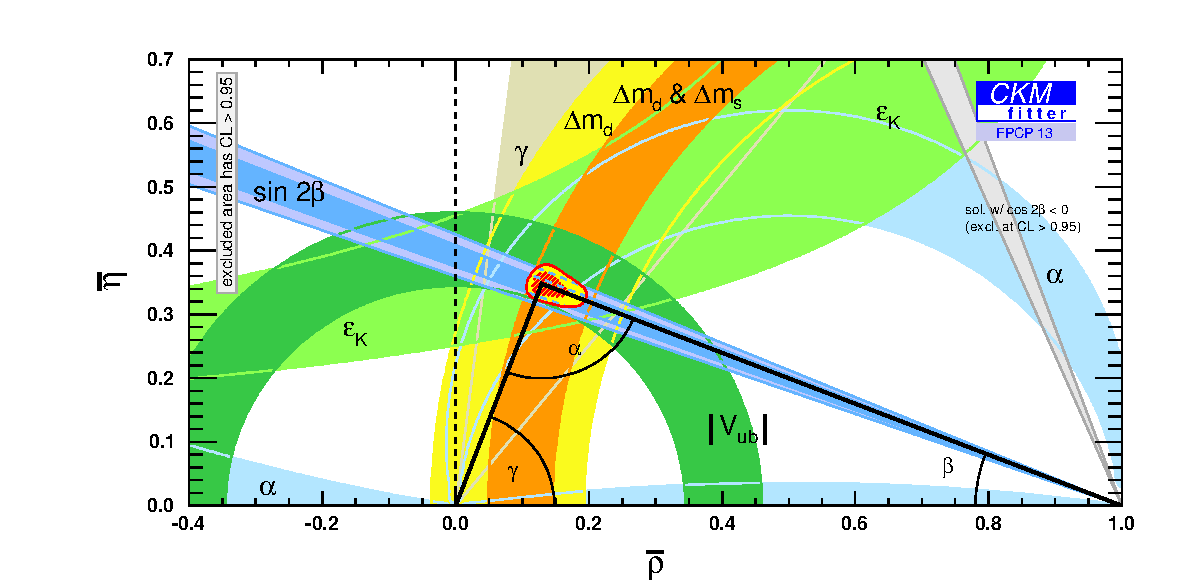
\includegraphics[trim=15mm 0mm 5mm 7mm, clip=true, width=\textwidth]{graphics/SM/rhoeta_small_global}
  \caption{Constraints on the d--b unitarity triangle resulting from the global Standard-Model fit by the CKMfitter Group
           \cite{Charles:2004jd}. The fit estimates the coordinates of the triangle apex in the complex plane, which is given by the
	   parameters $\rhobar\approx(1-\tfrac{1}{2}\lam^2)\,\rho$ and $\etabar\approx(1-\tfrac{1}{2}\lam^2)\,\eta$.
           Constraints on these parameters from the measurements that are input to the fit are shown as the coloured bands.}
  \label{fig:unitTriangleMeas}
\end{figure}

Quark-flavour changing interactions and the CKM picture of CP violation provide excellent probes for testing the Standard Model. There are,
for example, measurements that would yield one of the CKM angles if the Standard Model is a good description of the relevant physics
processes. If such a measurement gives a deviation from the value predicted by a global fit or from the value from another measurement,
this would be clear evidence for physics beyond the Standard Model.

The value of the angle $\bs$ is very small, since the imaginary part of $\Vts$ is proportional to a factor $\lam^2$, as was shown in
Equations~\ref{eq:CKMApprox} and \ref{eq:CKMBetasApprox}. A null test is therefore provided by measurement of an observable quantity that
is equal to $\bs$ in the Standard Model. Even if contributions of unknown new physics to such a quantity are small, they could still be
larger than the suppressed Standard-Model contribution. 

Sections~\ref{sec:introMixing} and \ref{sec:introDecay} give an introduction to the measurement of CP violation in the decay of the system
of $\Bs$ and $\Bsbar$ mesons into a $\Jpsi$ and a $\phimes$ meson. This measurement yields the phase $\phis$, which is approximately equal
to $-2\bs$ in the Standard Model. Testing the Standard Model with this CP-violation measurement is the main objective of this thesis.

In addition to the charge and parity operations there is the transformation of \emph{time reversal} (T), which inverts the time coordinate.
A fundamental assumption of quantum field theory is that all processes are invariant under a combined C, P and T transformation. The
Standard Model as well as the physics processes beyond the Standard Model that are discussed in this thesis are bound by this restriction.


%%%%%%%%%%%%%%%%%%%%%%%%%%%%%%%%%%%%%%
\subsection{Beyond the Standard Model}
%%%%%%%%%%%%%%%%%%%%%%%%%%%%%%%%%%%%%%


